\documentclass[landscape, 8pt]{extarticle}

\usepackage{../../preamble}
\usepackage[separate]{../../rss/thmboxes_v4}
\usepackage{symbols}


\begin{document}
\setlength{\abovedisplayskip}{3.5pt}
\setlength{\belowdisplayskip}{3.5pt}
\setlength{\abovedisplayshortskip}{3.5pt}
\setlength{\belowdisplayshortskip}{3.5pt}
\setlength{\multicolsep}{0pt}% 50% of original values
\setlist{topsep=3pt, itemsep=0pt}

\begin{multicols*}{3}
\raggedcolumns

\section*{\huge Algebraic Topology Notes}
Made by Leon :) \textit{Note: Any reference numbers are to the lecture notes}

\section{Introduction}
\setcounter{subsection}{1}

\begin{rcl}[Topology]{rcl:topology2}{}
	An \textbf{(open) topology} on $X$ is a collection of subsets $\tau \subset P(X)$ such that
	\begin{itemize-zero}
	    \item $\emptyset\in \tau$ and $X\in \tau$
	\end{itemize-zero}
	\begin{multicols}{2}
	\begin{itemize-zero}
		\item $\tau$ is closed under finite intersections: If $\{U_{1},\dots,U_{n}\} \subset \tau$ then
			\[\bigcap_{i=1,\dots,n} U_{i}\in \tau\]
		\item $\tau$ is closed under arbitrary unions: If $\{U_{1},. .,U_{n}\} \subset \tau$ is a family of open subsets then
			\[\bigcup_{i=1,\dots,n} U_{i}\in \tau\]
	\end{itemize-zero}
	\end{multicols}

	The subsets $U \in \mathcal{T}$ are called \textbf{open} and their complements in $X$ define \textbf{closed subsets}.
	\tcbline
	Two examples of a topology on a set $X$ are the following:
	\begin{itemize-tight}
	    \item The \textbf{Trivial Topology}: $\tau_{\mathrm{triv}} = \{\emptyset, X\}$
	    \item The \textbf{Discrete Topology}: $\tau_{\mathrm{dis}} = P(X)$
	\end{itemize-tight}
	\tcbline
	A subset $A \subset X$ is \textbf{clopen if it is both closed and open}
\end{rcl}

\begin{dfn}[Connected Spaces]{dfn:connected}{1}
	A topological space $X$ is \textbf{connected} if $X = A \cup B$ with $A,\,B \subset X$ open implies that $A = \emptyset$ or $A = X$.
\end{dfn}

\begin{ppn}[Connectedness and Clopens]{ppn:connected-clopen}{1}
	A topological space $X$ is \textit{connected} iff the only clopens are $\emptyset$ and $X$.
\end{ppn}

\begin{xmp}[Examples of Connected Topologies]{xmp:connected-topo-exmp}{1}
	\begin{itemize-zero}
	    \item Every $X$ with the trivial topology is connected.
	    \item Every $X$ with the discrete topology isn't connected unless $X = \emptyset$ or $X = \{\ast\}$ (in which it coincides with the trivial topology).
	    \item The real line $\mathbb{R}$ with the standard topology is connected.
	\end{itemize-zero}
\end{xmp}

\begin{ppn}[Continuous Maps]{ppn:contiuous-maps}{2}
	Let $f : X \to Y$ be a continuous map of topological spaces and let $X$ be connected. Then $f(X)$ is connected.
\end{ppn}

\begin{ppn}[Connected Equivalence Relation]{ppn:equivalence-relation}{3}
	For a topological space $X$, define $x \sim y$ if there exists some connected subset that contains both. The relation $x \sim y$ is an equivalence relation.
\end{ppn}

\vspace{-7pt}
\begin{dfn}[Connected Components]{dfn:connected-components}{2}
	The equivalence classes of this relation are called \textbf{connected components}. In particular, a space $X$ is connected iff it only has a single connected component.
\end{dfn}

\vspace{-7pt}
\begin{dfn}[Path]{dfn:path}{3}
	Let $I$ denote the closed unit interval $[0,1]$. A \textbf{path} in $X$ is a \newline continuous map $\alpha : I \to X$. The points $\alpha(0)\in X$ and $\alpha(1)\in X$ will be called \textbf{start} and \textbf{end} points respectively.

	We define a path relation between points in $X$ by declaring $x \sim y$ if there exists some path $\alpha : I \to X$ that starts at $x$ and ends in $y$, i.e. $\alpha(0) = x$ and $\alpha(1) = y$. This is an equivalence relation from the following properties:
	\begin{enumerate-zero}
	    \item \textbf{Constant Path}: For all $x\in X$ there exists the constant path $c_{x} : I \to X$ defined by $c_{x}(t)=x$ for all $t\in I$
	    \item \textbf{Path reversal}: Let $\alpha : I \to X$ be a path in $X$. Define its reversed path by
			\begin{equation}\label{eq:path-reversal}
				\overline{\alpha} : I \to X,\;\quad t \mapsto \alpha(1-t)
			\end{equation}
		\item \textbf{Path Concatenation}: Let $\alpha,\,\beta : I \to X$ be two paths in $X$ s.t. $\alpha(1) = \beta(0)$. Their concatenated path is defined by:
			\begin{equation}
				\alpha \ast \beta(t) := \begin{cases}
					\alpha(2t), &0 \le t\le 1 /2\\
					\beta(2t-1) & 1 /2 \le t \le 1
				\end{cases}
			\end{equation}
	\end{enumerate-zero}
\end{dfn}

\vspace{-7pt}
\begin{dfn}[Path-Connected Components]{dfn:path-connected-comps}{4}
	The equivalence classes are called \textbf{path-connected components} and their set is denoted by $\pi_{0}(X)$. A space $X$ is called \textbf{path-connected} if $\pi_{0}(X)$ is a one-point set, i.e. any two points $x,\,y$ can be related by a path in $X$.
\end{dfn}

\vspace{-7pt}
\begin{rem}[Random examples]{rem:random-examples}{1}
	The following statements are true:
	\begin{itemize-zero}
	    \item A homeomorphism $X \cong Y$ induces a bijection $\pi_{0}(X) \cong \pi_{0}(Y)$.
	    \item If $X$ is path-connected, it is also connected.
	    \item The \textit{topologist's sine curve} defined by $X = \{0\} \times [-1,1] \times \{(x,\,\sin(1 /x)) \mid 0 < x\}$ is connected but not path-connected.
	\end{itemize-zero}
\end{rem}

\vspace{-7pt}
\begin{dfn}[Homotopy]{dfn:homotopy}{5}
	\sbsadapt{
A \textbf{homotopy} of maps $f,\, g : X \to Y$ is a\newline continuous map $h : X \times I \to Y$ such that $h(-, 0) = f$ and $h(-, 1) = g$.
	}{
		% https://q.uiver.app/#q=WzAsMixbMCwwLCJYIl0sWzIsMCwiWSJdLFswLDEsImYiLDAseyJjdXJ2ZSI6LTJ9XSxbMCwxLCJnIiwyLHsiY3VydmUiOjJ9XSxbMiwzLCJoIiwwLHsic2hvcnRlbiI6eyJzb3VyY2UiOjIwLCJ0YXJnZXQiOjIwfX1dXQ==
		\begin{tikzcd}[ampersand replacement=\&,cramped]
			X \&\& Y
			\arrow[""{name=0, anchor=center, inner sep=0}, "f", curve={height=-12pt}, from=1-1, to=1-3]
			\arrow[""{name=1, anchor=center, inner sep=0}, "g"', curve={height=12pt}, from=1-1, to=1-3]
			\arrow["h", shorten <=3pt, shorten >=3pt, Rightarrow, from=0, to=1]
		\end{tikzcd}
	}
	If such a homotopy exists, $f$ is \textbf{homotopic} to $g$. This defines an equivalence relation $f \simeq g$ on the space of maps $\Map(X,\, Y)$.

	% TODO: the equivalence relation axioms
\end{dfn}

\vspace{-7pt}
\begin{xmp}[Paths as Homotopies]{xmp:path-homotopy}{2}
	Points in $X$ are the same as maps $\ast \to X$ from the one-point set $\ast$ to $X$. A path $\alpha : I \to K$ corresponds to a homotopy $\ast \times I \to X$.
\end{xmp}

\begin{rem}[Composition of Homotopies]{rem:homotopy-composition}{1.5}
	\begin{itemize-zero}
	    \item \textbf{Horizontal Composition}: Let $h, h' : X \times I \to Y$ be two homotopies in $X$ such that $h(-, 1) = h'(-, 0) : X \to Y$. Their concatenated homotopy is defined by
			\stepcounter{equation}
			\begin{equation}\label{eq:homotopy}
				h \ast h'(-, t) := \begin{cases}
				h(-, 2t) & 0 \le t \le 1 /2\\
				h'(-, 2t - 1) & 1 /2 \le t \le 1
			\end{cases}\end{equation}
		\item \textbf{Vertical Composition}: Let $h : X \times I \to Y$ and $k : Y \times I \to Z$ be two homotopies on maps from $X$ to $Y$, and $Y$ to $Z$. Then
			\begin{equation}
				k \circ h := [X \times I \prightarrow{\Id \times \Delta} X \times I^{2} \prightarrow{h \times \Id} Y \times I \prightarrow{k} Z]
			\end{equation}
			where $\Delta : I \to I^{2}$, $t \mapsto (t, t)$ is the diagonal map, or explicitly,
			\[k \circ h(x, t) = k(h(x, t), t)\]
	\end{itemize-zero}

	\sbsadapt
	{
% https://q.uiver.app/#q=WzAsMyxbMCwwLCJYIl0sWzIsMCwiWSBcXHNpbSBYIl0sWzQsMCwiWSJdLFswLDFdLFswLDEsImYiLDAseyJvZmZzZXQiOi0zLCJjdXJ2ZSI6LTF9XSxbMCwxLCJsIiwyLHsib2Zmc2V0IjozLCJjdXJ2ZSI6MX1dLFsxLDIsImYiLDAseyJvZmZzZXQiOi0zLCJjdXJ2ZSI6LTF9XSxbMSwyLCJsIiwyLHsib2Zmc2V0IjozLCJjdXJ2ZSI6MX1dLFszLDUsImgnIiwyLHsic2hvcnRlbiI6eyJzb3VyY2UiOjIwLCJ0YXJnZXQiOjIwfX1dLFs2LDcsImsnIFxcYXN0IGgiLDAseyJzaG9ydGVuIjp7InNvdXJjZSI6MjAsInRhcmdldCI6MjB9fV0sWzQsMywiaCIsMix7InNob3J0ZW4iOnsic291cmNlIjoyMCwidGFyZ2V0IjoyMH19XV0=
		\begin{tikzcd}[ampersand replacement=\&,cramped,column sep=scriptsize]
			X \&\& {Y\hspace{-0.2em}\sim\hspace{-0.2em}X} \&\& Y
			\arrow[""{name=0, anchor=center, inner sep=0}, from=1-1, to=1-3]
			\arrow[""{name=1, anchor=center, inner sep=0}, "f", shift left=3, curve={height=-8pt}, from=1-1, to=1-3]
			\arrow[""{name=2, anchor=center, inner sep=0}, "l"', shift right=3, curve={height=8pt}, from=1-1, to=1-3]
			\arrow[""{name=3, anchor=center, inner sep=0}, "f", shift left=3, curve={height=-8pt}, from=1-3, to=1-5]
			\arrow[""{name=4, anchor=center, inner sep=0}, "l"', shift right=3, curve={height=8pt}, from=1-3, to=1-5]
			\arrow["{h'}", shorten <=2pt, shorten >=2pt, Rightarrow, from=0, to=2]
			\arrow["h"', shorten <=2pt, shorten >=2pt, Rightarrow, from=1, to=0]
			\arrow["{k' \ast h}"', shorten <=3pt, shorten >=3pt, Rightarrow, from=3, to=4]
		\end{tikzcd}
	}
	{
% https://q.uiver.app/#q=WzAsNCxbMCwwLCJYIl0sWzIsMCwiWSJdLFs0LDAsIlogXFxzaW0gWCJdLFs2LDAsIloiXSxbMCwxLCJmIiwwLHsiY3VydmUiOi0yfV0sWzAsMSwiZyIsMix7ImN1cnZlIjoyfV0sWzEsMiwiZiciLDAseyJjdXJ2ZSI6LTJ9XSxbMiwzLCJmJyBcXGNpcmMgZiIsMCx7ImN1cnZlIjotMn1dLFsyLDMsImcnIFxcY2lyYyBnIiwyLHsiY3VydmUiOjJ9XSxbMSwyLCJnJyIsMix7ImN1cnZlIjoyfV0sWzQsNSwiaCIsMCx7InNob3J0ZW4iOnsic291cmNlIjoyMCwidGFyZ2V0IjoyMH19XSxbNiw5LCJrIiwwLHsic2hvcnRlbiI6eyJzb3VyY2UiOjIwLCJ0YXJnZXQiOjIwfX1dLFs3LDgsImsgXFxjaXJjIGgiLDAseyJzaG9ydGVuIjp7InNvdXJjZSI6MjAsInRhcmdldCI6MjB9fV1d
		\begin{tikzcd}[ampersand replacement=\&,cramped, column sep=small]
			X \&\& Y \&\& {Z\hspace{-0.2em}\sim\hspace{-0.2em}X} \&\& Z
			\arrow[""{name=0, anchor=center, inner sep=0}, "f", curve={height=-12pt}, from=1-1, to=1-3]
			\arrow[""{name=1, anchor=center, inner sep=0}, "g"', curve={height=12pt}, from=1-1, to=1-3]
			\arrow[""{name=2, anchor=center, inner sep=0}, "{f'}", curve={height=-12pt}, from=1-3, to=1-5]
			\arrow[""{name=3, anchor=center, inner sep=0}, "{g'}"', curve={height=12pt}, from=1-3, to=1-5]
			\arrow[""{name=4, anchor=center, inner sep=0}, "{f' \circ f}", curve={height=-12pt}, from=1-5, to=1-7]
			\arrow[""{name=5, anchor=center, inner sep=0}, "{g' \circ g}"', curve={height=12pt}, from=1-5, to=1-7]
			\arrow["h", shorten <=3pt, shorten >=3pt, Rightarrow, from=0, to=1]
			\arrow["k", shorten <=3pt, shorten >=3pt, Rightarrow, from=2, to=3]
			\arrow["{k \circ h}", shorten <=3pt, shorten >=3pt, Rightarrow, from=4, to=5]
		\end{tikzcd}
	}
\end{rem}

\begin{lma}[Concatenation Relation]{lma:concatenation-relation}{1}
	Let $f,\, f' : X \to Y$ and $g, g' : Y \to Z$ be maps such that $f \simeq f'$ and $g \simeq g'$. Then $g \circ f \simeq g' \circ f'$ as maps from $X$ to $Z$. In particular, $g' \circ f \sim g \circ f$ and $g \circ f' \sim g \circ f$.
\end{lma}

\begin{dfn}[Homotopy Equivalence]{dfn:homotopy-equivalence}{6}
	A map $f : X \to Y$ is called a \textbf{homotopy equivalence} if there exists a map $g : Y \to X$ and homotopies $f \circ g \simeq \Id_{Y},\, g \circ f \simeq \Id_{X}$. In other words, $g$ satisfies the properties of an inverse up to homotopy. It is called a \textbf{homotopy inverse} of $f$.
\end{dfn}

\begin{xmp}[Circle to \texorpdfstring{$\mathbb{R}^{2}$}{R2}]{xmp:circle-to-R2}{3}
	The inclusion map $\mathbb{S}^{1} \hookrightarrow \mathbb{R}^{2}$ is not a homotopy equivalence, but the inclusion $\mathbb{S}^{1} \hookrightarrow \mathbb{R}^{2} \backslash \{0\}$ is a homotopy equivalence.
\end{xmp}

\begin{ppn}[Unique Inverses of Homotopy]{ppn:homotopy-unique-inverse}{4}
	Homotopy inverses are unique up to homotopy.
\end{ppn}

\begin{dfn}[Homotopic Spaces]{dfn:homotopic-space}{7}
	Two spaces $X$ and $Y$ are called \textbf{homotopy equivalent}, or \textbf{of the same homotopy type}, and denoted by $X \simeq Y$ if there exists a homotopy equivalence $f : X \to Y$.
	\tcbline
	\textbf{Note}: $\cong$ for homeomorphisms and $\simeq$ for homotopy equivalence.
\end{dfn}

\begin{lma}[Composition of Inverses]{lma:inverse-composition}{2}
	Let $f : X \to y$, $g : Y \to Z$ with homotopy inverses $\overline{f} : Y \to X$ and $\overline{g} : Z \to Y$ respectively. Then $\overline{f} \circ \overline{g} : Z \to X$ is a homotopy inverse of $g \circ f : X \to Z$. In particular, $X \simeq Y$, $Y \simeq Z$ implies $X \simeq Z$.
\end{lma}

\section{Contractible Spaces}
\vspace{-5pt}
\begin{dfn}[Contractible Space]{dfn:contractible}{8}
	A space $X$ is called \textbf{contractible} if it is homotopy equivalent to a point, i.e. $X \simeq \ast$.
	\tcbline
	The \textbf{terminal map} is the unique map $X \to \ast$. Contractibility requires that there is a homotopy inverse of that map, i.e. a map $\ast \to x$ along with homotopies
	\begin{equation}\label{eq:contractibility}
		h : [\ast \to X \to \ast] \simeq \Id_{\ast},\quad k : [X \to \ast \to X] \simeq \Id_{X}
	\end{equation}
\end{dfn}

\begin{xmp}[Examples of Contractible Spaces]{xmp:contractible-example}{4}
	\begin{enumerate-zero}
	    \item $\mathbb{R}^{n}$ is contractible. Let $x_{0}$ be a fixed point in $\mathbb{R}^{n}$ and define the (straight line) homotopy $h : c_{x_{0}} \simeq \Id_{\mathbb{R}^{n}}$ by
			\[h(x, t) = (1 - t)x_{0} + tx.\]
		\item $\mathbb{S}^{n-1} \simeq \mathbb{R}^{n} \backslash \{0\}$. The inclusion $\mathbb{S}^{n-1} \hookrightarrow \mathbb{R}^{n}\backslash \{0\}$ and the shrinking map
			\vspace{-2pt}
			\[\mathbb{R}^{n}\backslash \{0\} \to \mathbb{S}^{n-1},\;\quad x \mapsto \frac{x}{\lvert x \rvert}\]
			\par\vspace{-7pt}
			are homotopy inverses.
	\end{enumerate-zero}
\end{xmp}

\begin{rem}[Remarks about Contractible Spaces]{rem:contractible}{3}
	\begin{enumerate-zero}
	    \item Contractible spaces are path-connected. Let $x_{0}$ be the point where the space $X$ contracts to. In particular, we are given with a homotopy $h : c_{x_{0}} \simeq \Id_{X}$. For any $x\in X$, the map $h(x, -) : I \to X$ defines a path from $x_{0}$ to $x$ and thus every element $x\in X$ is path-connected to $x_{0}$.
	    \item The converse does not hold, for example $X = \mathbb{S}^{1}$.
	    \item A contractible space $X$ is contractible at any point $x_{0}$. $X$ is path-connected, so a path $x$ to $x'$ defines a homotopy $c_{x} \simeq c_{x'}$.
	    \item Any two maps $f,\,g : X \to Y$ are homotopic if $Y$ is contractible.
	\end{enumerate-zero}
\end{rem}

\begin{dfn}[Retracts and Deformation Retracts]{dfn:retracts}{9}
	\begin{itemize-zero}
	    \item A \textbf{retract} of $X$ onto a subspace $A \subset X$ is a map $r : X \to A$ such that $r \rvert_{A} = \Id_{A}$. Equivalently, this is a map $r : X \to X$ such that $r^{2} = r$ and $r(X) = A$.
	    \item A \textbf{deformation retract} of $X$ onto $A$ is the additional datum of a homotopy $h : \Id_{X} \simeq i \circ r$.
	\end{itemize-zero}
	In other words, a deformation retract is a homotopy $h : X \times I \to X$ such that $h(x, 0) = x$ and $h(x, 1) \in A$ for all $x\in X$ and $h(a, 1) = a$ for all $a\in A$. Not all retracts can form deformation retracts. For instance, the retract $X$ onto a point $\{x_{0}\}$ can be a deformation retract iff $X$ is contractible.
\end{dfn}

\begin{rem}[Strong vs Weak Deformation Retracts]{rem:strong-weak-retracts}{4}
	This notion is called \textbf{weak} deformation retract. A \textbf{strong} deformation retract has the condition $h(a, t) = a$ for all $t\in I,\, a\in A$. Our notion of a (weak) deformation retract deforms $X$ into $A$ while allowing to deform $A$ to do so, while a strong deformation retract deforms $X$ into $A$ while keeping $A$ fixed at all times
\end{rem}

\begin{ppn}[Deformation Retracts and Homotopies]{ppn:deformation-homotopy}{5}
	A deformation retract of $X$ onto $A$ induces a homotopy equivalence $X \simeq A$.
\end{ppn}

\begin{rcl}[Quotient Space]{rcl:quotient-space}{2}
	Let $X$ be a topological space and let $\sim$ be an equivalence relation on $X$. Then, $X / \sim$ is equipped with the quotient topology and called a \textbf{quotient space}. If $Z$ is a closed subset in $X$, then we can also define the quotient space $X / Z$.
	\tcbline
	Another form of quotient spaces: Let $f : Z \to Y$ be a continuous map between a closed subset $Z \subset X$ and $Y$. Then
	\[X \cup_{f} Y = X \cup Y /z \sim f(z).\]
\end{rcl}

\begin{xmp}[Examples of Quotient Spaces]{xmp:quotient-spaces}{5}
	\begin{itemize-zero}
	    \item The quotient of the $n$-dimensional closed disk by its boundary is the $n$-sphere, i.e. $\mathbb{D}^{n} /\partial \mathbb{D}^{n} \cong \mathbb{S}^{n}$.
	    \item The $2$-torus: $\mathbb{R}^{2} / \mathbb{Z}^{2}$.
		\item The projective space: $\mathbb{RP}^{n} = \mathbb{R}^{n+1} \backslash \{0\} / \sim$ by the relation $x \sim y$ iff there exists some $\lambda\in \mathbb{R}^{\times}$ such that $x = \lambda y$. This corresponds to the space of lines through the origin in $\mathbb{R}^{n+1}$.
	\end{itemize-zero}
\end{xmp}

\begin{dfn}[Mapping Quotients]{dfn:mapping-quotients}{10}
	Let $f : X \to Y$ be a continuous map.
	\begin{itemize-zero}
	    \item Its \textbf{mapping cylinder} is defined as the topological space
			\[M_{f} := ( X \times I ) \cup Y / \sim\]
			where the quotient identifies $(x, 0) \sim f(x)$ for any $x\in X$.
			\vspace{3pt}
		\begin{multicols}{2}
		\item Its \textbf{cone} is the further \newline quotient:
			\[C_{f} = M_{f} /X \times \{1\}.\]
		\item The \textbf{cone} of a topological space $X$ is
			\[C_{X} := C_{\Id_{X}} = X \times I /X \times \{1\}.\]
		\end{multicols}
	\end{itemize-zero}
	\tcbline
	\vspace{-2pt}
	\sbsadapt{
	In other words, the mapping cylinder of $f : X \times Y$ is the pushout of the diagram:
	}
	{
	% https://q.uiver.app/#q=WzAsNCxbMCwwLCJYIFxcdGltZXMgXFx7MFxcfSJdLFsyLDAsIlkiXSxbMiwyLCJNX2YiXSxbMCwyLCJYIFxcdGltZXMgSSJdLFswLDEsImYiXSxbMSwyXSxbMCwzXSxbMywyXV0=
	\begin{tikzcd}[ampersand replacement=\&,cramped, column sep=small, row sep=small]
		{X \times \{0\}} \&\& Y \\
		\\
		{X \times I} \&\& {M_f}
		\arrow["f", from=1-1, to=1-3]
		\arrow[from=1-1, to=3-1]
		\arrow[from=1-3, to=3-3]
		\arrow[from=3-1, to=3-3]
	\end{tikzcd}
	}
\end{dfn}

\vspace{-2pt}
\begin{xmp}[Spheres]{xmp:spheres}{5.5}
	For $\mathbb{S}^{n}$ with the standard embedding $\mathbb{R}^{n+1} \backslash \{0\}$, the following map is a retract, because if $x$ has norm $\lvert x \rvert = 1$, then $r(x) = x$.
	\[r : \mathbb{R}^{n+1} \backslash \{0\} \to \mathbb{S}^{n},\;\quad x \mapsto \frac{x}{\lvert x \rvert}\]
	 For a deformation retract one needs to find a homotopy $h : i \circ r \simeq \Id_{X}$. We use the following straight-line homotopy:
	\[h : \mathbb{R}^{n+1} \backslash \{0\} \times I \to \mathbb{R}^{n+1} \backslash \{0\},\;\quad (x, t) \mapsto (1-t) \frac{x}{\lvert x \rvert} + tx.\]
	Indeed, $h(x, 0) = r(x)$ and $h(x, 1) = x$ for all $x$.
\end{xmp}

\begin{dfn}[Star-Shaped Spaces]{dfn:star-spaces}{11}
	A subset $S \subset \mathbb{R}^{n}$ is called \textbf{star-shaped} at a point $x_{0}\in S$, if for any $x\in S$ the line segment from $x_{0}$ to $x$ is contained in $S$, i.e.
	\[\{(1-t)x_{0} + tx \mid t\in [0,1]\} \subset S\]
	If $S$ is star-shaped at every point, then it is called \textbf{convex}.
\end{dfn}

\begin{xmp}[Star-Shaped Spaces are Contractible]{xmp:star-shaped-contractible}{5.6}
	%TODO: also show that they are path-connected
	Let $S$ be star-shaped at $x_{0}$ and $i : \{x_{0}\} \leftrightarrow S : r$ be the inclusion and constant maps. Define the straight line homotopy
	\[h : S \times I \to S,\;\quad (x, t) \mapsto (1 - t) x_{0} + tx\]
	which is well-defined by the star-shaped condition. Moreover, $h(x,0) = x_{0} = r(x)$ and $h(x,1) = x$ for all $x$. Hence, star-shaped, and in particular convex spaces, are contractible.
\end{xmp}

\begin{xmp}[M\"obius band]{xmp:mobius-band}{5.7}
	The M\"obius band $M$ can be defined as
	\[M = I^{2} / \sim\]
	where $\sim$ identifies the two vertical edges of $I^{2}$ by flipping one, \newline i.e. $(0, b) \sim (1,1-b)$ for $b\in I$. Its core $C \subset M$ is the line $\{[a, 1 /2] \mid a\in I\}$. Thus, the core is homeomorphic to $\mathbb{S}^{1}$. The M\"obius band deformation retracts onto its core, e.g. the retract $r : M \to C$ defined by $r([a, b]) := [(a, 1 /2)]$ and the homotopy
	\[h : M \times I \to M,\;\quad ([(a, b)], t) \mapsto \left[\left(a, (1-t) \frac{1}{2} + ^{}_{}\right)\right].\]
	In particular, $M \simeq \mathbb{S}^{1}$.
\end{xmp}

\begin{ppn}[Retracts of the Mapping Cylinder]{ppn:mapping-cylinder-retract}{6}
	Via Definition \href{dfn:mapping-quotients}{10}, the mapping cylinder is formed by the cylinder of $X$ by gluing $Y$ onto the bottom with the map $f$.

	The mapping cylinder $M_{f}$ strongly deformation retracts onto $Y$.

	\tcblower
	\begin{proof}
		Consider the retract:
		\[r:M_{f} \to Y\]
		defined by $r([x, s]) := [(x, 0)] = [f(x)]$ on the class of $(x, s) \in X \times I$ and $r([y]) = y$ for $y\in Y$. This is well-defined and by definition a retract on $Y$. Define the homotopy
		\[h : M_{f} \times I \to M_{f}\]
		by $h([(x, s)], t) := [(x, st)]$ for $(x, s)\in X \times I$ and $t\in I$, and by $h([y], t) := y$ for $y\in Y$. In particular, $h(-, 0) i \circ r$ and $h(-, 1) = \Id_{M_{f}}$. This forms a strong deformation retract.
	\end{proof}
\end{ppn}

\begin{rem}[Continuous Maps are Homotopic]{rem:continuous-map-homotopic}{6}
	\sbsadapt
	{
	Any continuous $f : X \to Y$ can be replaced up to homotopy equivalence by the closed inclusion $X\hspace{-0.1ex}\hookrightarrow \hspace{-0.1ex}M_{f},\, \hspace{-0.1ex}x \mapsto \hspace{-0.1ex}[(x, 1)]$. More precisely, it factorises through an inclusion and a homotopy equivalence as the following diagram commutes:
	}
	{
% https://q.uiver.app/#q=WzAsMyxbMCwwLCJYIl0sWzQsMCwiWSJdLFsyLDIsIk1fZiJdLFswLDEsImYiXSxbMCwyLCIiLDIseyJzdHlsZSI6eyJ0YWlsIjp7Im5hbWUiOiJob29rIiwic2lkZSI6InRvcCJ9fX1dLFsyLDEsIlxcc2ltZXEiLDJdXQ==
	\begin{tikzcd}[ampersand replacement=\&,cramped, column sep=tiny, row sep=small]
		X \&\&\&\& Y \\
		\\
		\&\& {M_f}
		\arrow["f", from=1-1, to=1-5]
		\arrow[hook, from=1-1, to=3-3]
		\arrow["\simeq"', from=3-3, to=1-5]
	\end{tikzcd}
}
\end{rem}

\begin{dfn}[Relative Homotopy]{dfn:relative-homotopy}{12}
	Let $X, Y$ be topological spaces and $A \subset X$ a subset in $X$. A homotopy $h : X \times I \to y$ is called \textbf{relative to $A$} if $h(a, t)$ is independent of $t$ for all $a\in A$. In particular, this defines homotopies between maps $f,\, g: X \to Y$ such that $f \rvert_{A} = g \rvert_{A}$.

	\tcbline
	This definition generalises ordinary homotopies, as an ordinary homotopy is the same as a homotopy relative to $\emptyset$.
\end{dfn}

\vspace{-7pt}
\begin{xmp}[Relative Homotopies and Retracts]{xmp:relative-retract}{6}
	A strong deformation retract of $X$ onto $A$ is a deformation retract such that the homotopy $h : i \circ r \simeq \Id_{X}$ is relative to $A$.
\end{xmp}

\vspace{-7pt}
\begin{dfn}[Homotopic Path]{dfn:homotopic-path}{13}
	Let $\alpha, \beta : I \to X$ be paths in $X$ such that $\alpha(0) = \beta(0)$ and $\alpha(1) = \beta(1)$. A relative homotopy from $\alpha$ to $\beta$ is a homotopy $h : I \times I \to x$ relative to $\partial I = \{0,1\}$, i.e.
	\begin{equation}
		h(-, 0) = \alpha, \quad h(-, 1) = \beta
	\end{equation}
	\par\vspace{-3pt}
	and
	\begin{equation}
		h(0, t) = \alpha(0) = \beta(0), \quad h(1,t)=\alpha(1)=\beta(1), \quad \forall t\in I.
	\end{equation}
	\tcbline
	In particular, at any point $t\in I$ a relative homotopy $h$ defines a path $h_{t} := h(-, t) : I \to X$ with start $\alpha(0) = \beta(0)$ and end $\alpha(1) = \beta(1)$. If one omits the relative condition, the start and end points of $h_{t}$ would be allowed to vary.
\end{dfn}

\vspace{-7pt}
\begin{rem}[Ordinary Homotopies and Paths]{rem:ordinary-homotopy-path}{7}
	Ordinary homotopies are not well suited for paths: Any path $\alpha : I \to X$ is homotopic (rel. $\emptyset$) to a constant - as the homotopy
	\[h : I \times I \to X, \quad (s, t) \mapsto \alpha(st)\]
	defines a homotopy from the constant path $c_{\alpha(0)}$ on $\alpha(0)$ to $\alpha$, i.e. $c_{\alpha(0)}\simeq \alpha$. Hence, (ordinary) homotopy classes of paths in $X$ are in $1$-to-$1$ correspondence with path-connected components of $X$.
\end{rem}

\vspace{-7pt}
\begin{ppn}[Homotopic Properties of Paths]{ppn:path-concatenation-homotopic}{7}
	Path concatenation is \textbf{unital}, \textbf{associative}, and \textbf{invertible} up to homotopy in the following sense: Let $\alpha,\, \beta,\, \gamma : I \to x$ be paths such that $\alpha(1) = \beta(0)$ and $\beta(1) = \gamma(0)$. Then there exists homotopies relative to $\{0,1\}$:
	\vspace{-2pt}
	\begin{enumerate}[noitemsep]
	    \item \textbf{Left Unitality}: $c_{\alpha(0)} \ast \alpha \simeq \alpha$
	    \item \textbf{Right Unitality}: $\alpha \simeq c_{\alpha(0)} \ast \alpha $
	    \item \textbf{Associativity}: $(\alpha \ast \beta) \ast \gamma \simeq \alpha \ast (\beta \ast \gamma)$
	    \item \textbf{Right Inverse}: $\alpha \ast \overline{\alpha} \simeq c_{\alpha(0)}$
	    \item \textbf{Left Inverse}: $\overline{\alpha} \ast \alpha \simeq c_{\alpha(1)}$
	\end{enumerate}
	\vspace{-2pt}
	where $c_{x}$ for some $x\in X$ denotes the constant path on $x$ and $\overline{\alpha}$ is the reversed path.
\end{ppn}

\vspace{-7pt}
\begin{lma}[]{lma:concat-relative-i}{3}
	Let $\alpha : I \to X$ be a path and $\lambda : I \to I$ a boundary preserving map, i.e. $\lambda(0) = 0$ and $\lambda(1)=1$. Then,
	\[\alpha \circ \lambda \simeq \alpha, \quad \text{rel.}\, \partial I.\]
\end{lma}

\begin{dfn}[Fundamental Group]{dfn:fundamental-group}{14}
	\vspace{-2pt}
	Let $X$ be a topological space and $x_{0}\in X$ some fixed point. The \textbf{fundamental group} of $X$ at $x_{0}$ is the group of homotopy classes of paths in $X$ that start and end on $x_{0}$. i.e. $\alpha : I \to X$ such that $\alpha(0) = \alpha(1) = x_{0}$, i.e.
	\vspace{-2pt}
	\[\pi_{1}(X, x) = \{\alpha : I \to X \mid \alpha(0) = \alpha(1)\} /\sim.\]
\end{dfn}

\vspace{-7pt}
\begin{thm}[Defining the Fundamental Group]{thm:fundamental-group-is-a-group}{1}
	\vspace{-2pt}
	The fundamental group $\pi_{1}(X, x_{0})$ is a well-defined group with:
	\begin{itemize-tight}
	    \item \textbf{Multiplication}: $[\alpha] \cdot [\beta] := [\alpha \ast \beta]$
			\begin{multicols}{2}
			\item \textbf{Unit}: $1 = [c_{x_{0}}]$
			\item \textbf{Inverse}: $[\alpha]^{-1} = [\overline{\alpha}]$
			\end{multicols}
	\end{itemize-tight}
\end{thm}

\vspace{-7pt}
\begin{lma}[Relative Concated Homotopic Paths]{lma:relative-concat-homo-path}{4}
	\vspace{-2pt}
	Let $\alpha \simeq \alpha' : I \to X$ and $\beta \simeq \beta' : I \to X$ be two pairs of relative homotopic paths such that $\alpha(1) = \alpha'(1) = \beta(0) = \beta'(0)$. Then the concatenations are relative homotopic, i.e.
	\vspace{-2pt}
	\[\alpha \ast \beta \simeq \alpha' \ast \beta', \quad \mathrm{rel. } \{0,1\}.\]
\end{lma}

\vspace{-7pt}
\begin{ppn}[Fundamental Group is Point Independent]{ppn:fundamental-group-point-independent}{8}
	\vspace{-2pt}
	Let $\gamma : I \to X$ be a path from $\gamma(0) = x$ to $\gamma(1) = x'$. Then it\newline induces a group isomorphism:
	\[(\gamma)_{\#} : \pi(X, x) \to \pi(X, x'),\;\quad [\alpha] \mapsto [\overline{\gamma} \ast \alpha \ast \gamma].\]
	\par\vspace{-4pt}
	\tcbline
	We abuse notation to say that for a path-connected space $X$, $\pi_{1}(X)$ is the fundamental group omitting the choice of base point.
\end{ppn}

\vspace{-7pt}
\begin{xmp}[Examples of Fundamental Groups]{xmp:fundamental-groups}{7}
	\vspace{-2pt}
	\begin{itemize-tight}
	    \item \textbf{Euclidean}: $\pi_{1}(\mathbb{R}^{n}) \cong 1$.
	    \item \textbf{Circle}: $\pi_{1}(\mathbb{S}_{1}) \cong \mathbb{Z}$.
	    \item \textbf{$n$-Spheres}: $\pi_{1}(\mathbb{S}^{n}) \cong 1$ for $n \ge 2$.
	    \item \textbf{Torus}: $\pi_{1}(\mathbb{S}^{1} \times \mathbb{S}^{1}) \cong \mathbb{Z} \oplus \mathbb{Z}$.
	    \item \textbf{Projective Spaces}: $\pi_{1}(\mathbb{RP}^{n}) \cong \mathbb{Z}_{2}$ for $n \ge 2$.
	\end{itemize-tight}
\end{xmp}

\vspace{-7pt}
\begin{dfn}[Pointed Space]{dfn:pointed-space}{15}
	\vspace{-2pt}
	\begin{itemize-zero}
	    \item A \textbf{pointed space} is a pair $(X, x)$ consisting of a topological space $X$ and a point $x\in X$.
	\vspace{-2pt}
	    \item A \textbf{map of pointed spaces} $f : (X, x) \to (Y, y)$ is a continuous map $f : X \to Y$ such that $f(x) = y$.
	\vspace{-2pt}
	    \item The \textbf{space of pointed maps} from $(X, x)$ to $(Y, y)$ is denoted
			\[\Map_{\ast}((X, x),\, (Y, y)) \subset \Map(X, Y).\]
	\end{itemize-zero}
	% TODO: explain this
\end{dfn}

\vspace{-7pt}
\begin{ppn}[Point and Path Space Isormophism]{ppn:point-path-iso}{9}
	\vspace{-2pt}
	We have a group isomorphism:
	\[\pi_{1}(X, x) \cong \pi_{0}(\Omega X).\]
	\par\vspace{-2pt}
	Similarly, one can iteratively define the $n$-fold loop space
	\[\Omega^{n}X := \Omega \Omega^{n-1}X = \Omega \cdots \Omega X\]
	\par\vspace{-2pt}
	There is a homeomorphism
	\[\Omega^{n}X \cong \Map_{\ast}((\mathbb{S^{n}}, 1),\,(X, x))\]
\end{ppn}

\begin{dfn}[\texorpdfstring{$n$}{n}-th Homotopy Group]{dfn:nth-homotopy-group}{16}
	The $n$-th homotopy group $\pi_{n}(X, x)$ is defined by:
	\[\pi_{n}(X, x) := \pi_{0}(\Omega^{n} X) \cong \pi_{0}(\Map_{\ast}(\mathbb{S}^{n}, (X, x))).\]
\end{dfn}

\vspace{-7pt}
\begin{dfn}[Simply Connected Space]{dfn:simply-connected-space}{17}
	A path-connected space $X$ is called \textbf{simply connected} if its fundamental group is trivial, i.e.
	\vspace{-4pt}
	\[\pi_{1}(X) = 1\]
	\par\vspace{-4pt}
	\tcbline
	Some examples are $\mathbb{R}^{n}$, $\mathbb{S}^{n}$ for $n > 1$, and some non-examples are $\mathbb{S}^{1}$, $\mathbb{S}^{1} \times \mathbb{S}^{1}$ and $\mathbb{RP}^{2}$.
\end{dfn}

\vspace{-7pt}
\begin{thm}[Fundamental Group Isomorphism]{thm:homotopy-isomorphism}{2}
	Let $f : X \to Y$ be a homotopy equivalence and $x\in X$ an arbitrary base point. Then, the map:
	\[f_{\ast} : \pi_{1}(X, x) \to \pi_{1}(Y, f(x)),\;\quad [\alpha] \mapsto [f \circ \alpha]\]
	In particular, for homotopy equivalent spaces $X \simeq Y$ which are path-connected, we get $\pi_{1}(X) \cong \pi_{1}(Y)$.
	\tcbline
	A map of pointed spaces $f : (X, x) \to (Y, y)$ is a \textbf{homotopy equivalence of pointed spaces} or \textbf{homotopy equivalence relative $\{x\}$} if there exists a map of pointed spaces $g : (Y, y) \to (X, x)$ along with relative homotopies
	\[h : f \circ g \simeq \Id_{Y} \quad \text{rel. } \{y\}\]
	and
	\[k : g \circ f \simeq \Id_{X} \quad \text{rel. } \{x\}\]
\end{thm}

\vspace{-7pt}
\begin{xmp}[Strong Deformation Retracts Homotopies]{xmp:strong-deformation-homotopy}{9}
	A strong deformation retract of $X$ onto a subspace $A$ gives a homotopy equivalence of pointed spaces $(x, a) \to (A, a)$ for any choice of $a\in A$. In particular, a contractible space $X \simeq \ast$ determines a homotopy equivalence of pointed spaces $(X, x) \to \ast$ for any choice of base point $x$.
\end{xmp}

\vspace{-7pt}
\begin{lma}[Pointed Space Isomorphism]{lma:pointed-space-isomorphism}{5}
	Let $f : (X, x) \to (Y, y)$ be a homotopy equivalence of pointed spaces. Then the map
	\[f_{\ast} : \pi_{1}(X, x) \to \pi_{1}(Y, y)\]
	is a group isomorphism.

	\tcbline
	\textbf{Corollary 1}: Let $r : X \to A$ be a strong deformation retract of $X$ onto $A \subset X$. Then for any $a\in A$,
	\vspace{-4pt}
	\[\pi_{1}(X, a) \cong \pi_{1}(A, a)\]
	\par\vspace{-2pt}
	In particular, contractible spaces are simply connected.
\end{lma}

\vspace{-7pt}
\begin{lma}[Identity Homomorphic Isormorphism]{lma:id-homo-iso}{6}
	Let $f : X \to X$ be a continuous map which is homotopic to $\Id_{X}$. Then, the map
	\[f_{\ast} : \pi_{1}(X, x_{0}) \to \pi_{1}(X, f(x_{0}))\]
	is a group isomorphism for any choice of base point $x_{0}\in X$.
\end{lma}

\begin{dfn}[Homotopy Lifting Property]{dfn:homotopy-lifting-property}{18}
	\sbsadapt{A continuous map $p : E \to X$ satisfies the \textbf{homotopy lifting property} (HLP) with respect to a topological space $Y$ if for any commuting diagram:}
	{
	% https://q.uiver.app/#q=WzAsNCxbMCwwLCJZIFxcdGltZXMgXFx7MFxcfSJdLFsyLDAsIkUiXSxbMiwyLCJYIl0sWzAsMiwiWSBcXHRpbWVzIEkiXSxbMCwxLCJIXzAiXSxbMSwyLCJwIl0sWzAsMywiIiwyLHsic3R5bGUiOnsidGFpbCI6eyJuYW1lIjoiaG9vayIsInNpZGUiOiJ0b3AifX19XSxbMywyLCJoIl0sWzMsMSwiXFxleGlzdHMiLDAseyJzdHlsZSI6eyJib2R5Ijp7Im5hbWUiOiJkYXNoZWQifX19XV0=
		\begin{tikzcd}[ampersand replacement=\&,cramped, column sep=small, row sep=scriptsize]
			{Y \times \{0\}} \&\& E \\
			\\
			{Y \times I} \&\& X
			\arrow["{H_0}", from=1-1, to=1-3]
			\arrow[hook, from=1-1, to=3-1]
			\arrow["p", from=1-3, to=3-3]
			\arrow["\exists", dashed, from=3-1, to=1-3]
			\arrow["h", from=3-1, to=3-3]
		\end{tikzcd}
	}
	
	There exists a map $H : Y \times I \to E$ s.t. both triangles commute, i.e. $H \rvert_{Y \times \{0\}} = H_{0}$ and $p \circ H = h$.

	\tcbline
	The map $p : E \to X$ has the HLP if for any homotopy $h : Y \times I \to X$ of maps $h(-, 0) := f_{0}$ and $h(-, 1) := f_{1}$ of maps $Y \to X$ and a choice of lift $H_{0}$ of $f_{0}$, then the homotopy $h$ lifts to a homotopy $H : Y \times I \to E$. In particular, if $f_{0} \simeq f_{1} : Y \to X$ and $H_{0}$ is a lift of $f_{0}$, we find $H_{0} \simeq H_{1}$ where $H_{1}$ lifts $f_{1}$.
	\tcbline
	\textbf{Example 10}: The identity map $\Id_{X} : X \to X$ has the HLP with respect to any space $Y$.
\end{dfn}

\begin{dfn}[Covering Space]{dfn:covering-space}{19}
	A \textbf{covering space} of $X$ is a topological space $\overline{X}$ along with a continuous map $p : X \to x$ such that for any point $x\in X$ there exists an open neighbourhood $U \subset X$ whose preimage $p^{-1}(U) = \bigcup_{j\in J} V_{j}$ and the opens $V_{j} \subset \overline{X}$ map homeomorphically to $U$ under $p$. In other words, a covering space of $X$ looks locally like a product of $X$ with a discrete space.
\end{dfn}

\begin{xmp}[Example of a Covering Space]{xmp:covering-space}{11}
	\begin{enumerate-zero}
	    \item The projection map $p : X \times Z \to X$ is a covering map if $Z$ is a discrete topological space. If $Z$ is not discrete, then this is not a covering map in general.
	    \item The identity map $\Id_{X} : X \to X$ is trivially a covering map.
	    \item While the projection of $p : X \times I \to X$ from the cylinder is not a covering map, its restriction to the boundary $\partial(X \times I ) = X \times \{0, 1\} =: \overline{X}$ gives a trivial ($2$-fold) cover of $X$.
	    \item Recall that the M\"obius band $M$ deformation retracts onto its core $\mathbb{S}^{1}$. Restricting to the boundary $\partial M = \mathbb{S}^{1}$, one obtains a (non-trivial) covering map $\mathbb{S}^{1}\to \mathbb{S}^{1}$. This map coincides with $z \mapsto z^{2}$ if we identify $S^{1}$ as the unit circle in $\mathbb{C}$.
	\end{enumerate-zero}
\end{xmp}

\begin{thm}[Unique HLPs from Covering Maps]{thm:covering-unique-hlp}{3}
	\sbsadapt{Let $p : \tilde{X} \to X$ be a covering map and $Y$ any topological space. Then $p$ \newline satisfies the HLP uniquely:

	i.e. the lift $H$ not only exists, but it is also unique.}
	{
% https://q.uiver.app/#q=WzAsNCxbMCwwLCJZIFxcdGltZXMgXFx7MFxcfSJdLFsyLDAsIlxcdGlsZGV7WH0iXSxbMiwyLCJYIl0sWzAsMiwiWSBcXHRpbWVzIEkiXSxbMCwxLCJIXzAiXSxbMSwyLCJwIl0sWzAsMywiIiwyLHsic3R5bGUiOnsidGFpbCI6eyJuYW1lIjoiaG9vayIsInNpZGUiOiJ0b3AifX19XSxbMywyLCJoIl0sWzMsMSwiXFxleGlzdHMhIiwwLHsic3R5bGUiOnsiYm9keSI6eyJuYW1lIjoiZGFzaGVkIn19fV1d
\begin{tikzcd}[ampersand replacement=\&,cramped]
	{Y \times \{0\}} \&\& {\tilde{X}} \\
	\\
	{Y \times I} \&\& X
	\arrow["{H_0}", from=1-1, to=1-3]
	\arrow[hook, from=1-1, to=3-1]
	\arrow["p", from=1-3, to=3-3]
	\arrow["{\exists!}", dashed, from=3-1, to=1-3]
	\arrow["h", from=3-1, to=3-3]
\end{tikzcd}
	}
	
\end{thm}

\columnbreak
% TODO: wtf?
\begin{crl}[]{crl:something-pathy}{2}
	\begin{enumerate-zero}
	    \item Let $\gamma : I \to X$ be a path and fix a point $\tilde{x_{0}}\in \tilde{X}$ such that $p(\tilde{x_{0}}) = \gamma(0)$. Then, there exists a unique path $\tilde{\gamma} : I \to \tilde{X}$ which starts at $\tilde{x_{0}}$ and lifts $\gamma$ i.e. $p \circ \tilde{\gamma} = \gamma$
	    \item Let $h : I \times I \to X$ be a (relative) homotopy of paths $h(-, 0) =: \gamma_{0}$ and $h(-, 1) =: \gamma_{1}$, and fix a point $\tilde{x_{0}}$ such that $p(\tilde{x_{0}}) = h(0, t) = \gamma_{0}(0) = \gamma_{1}(0)$. Suppose $\tilde{\gamma_{0}} : I \to X$ is a lift of $\gamma$ starting at $\tilde{\gamma_{0}}(0) = \tilde{x_{0}}$. Then, there exists a unique homotopy of paths $\tilde{h} : I \times I \to \tilde{X}$ which lifts $h$ and $\tilde{h}(-, 0) = \tilde{\gamma_{0}}$
	\end{enumerate-zero}
\end{crl}

\begin{thm}[Fundamental Groups]{thm:fundamental-group-thms}{4-7}
	\begin{itemize-zero}
		\item \textbf{Theorem 4}: The fundamental group of the circle is $\pi_{1}(\mathbb{S}^{1}) \cong \mathbb{Z}$. It is generated by the class of
			\[\alpha : I \to \mathbb{S}^{1},\;\quad t \mapsto e^{2\pi i t}.\]
			\par\vspace{-5pt}
		\item \textbf{Theorem 5 (Brouwer's Fixed Point Theorem)}: Any continuous map $f : \mathbb{D}^{2} \to \mathbb{D}^{2}$ has a fixed point, i.e. there exists $x \in \mathbb{D}^{2}$ such that $f(x) = x$.
		\item \textbf{Theorem 6 (Fundamental Theorem of Algebra)}: Every non-constant complex polynomial $p\in \mathbb{C}[z]$ has at least one root, i.e. $p(z_{0}) = 0$ for some $z_{0}$.
		\item \textbf{Theorem 7}: Fundamental Group of $\mathbb{S}^{n}$: The fundamental group of $\mathbb{S}^{n}$ is trivial for $n \ge 2$, i.ke. $\pi_{1}(\mathbb{S}^{2}) \cong 1$ for $n \ge 2$
	\end{itemize-zero}
\end{thm}

\begin{lma}[Closed Paths Homotopic to Loops]{lma:closed-path-loop}{7}
	Let $(X, x_{0})$ be a topological space with an open cover $\{U_{j}\}_{j\in J}$ such that $U_{j}$ are path-connected neighbourhoods of $x_{0}$ and $U_{j} \cap U_{j'}$ is path-connected for any $j, j' \in J$. Then, any closed path $\gamma$ based at $x_{0}$ is homotopic to a concatenation $\gamma_{1} \ast \gamma_{2} \ast \cdots \ast \gamma_{n}$ of loops at $x_{0}$ each of them contained in a single $U_{j}$
\end{lma}

\begin{crl}[Homemorphisms between \texorpdfstring{$\mathbb{R}^{2}$}{R2} and \texorpdfstring{$\mathbb{R}^{n}$}{Rn}]{crl:rn-homeomorphism}{3}
	There is no homeomorphism between $\mathbb{R}^{2}$ and $\mathbb{R}^{n}$ for $n \ne 2$
\end{crl}

% TODO: proof
% TODO: the remark

\begin{rcl}[Defining the Real Projective Space]{rcl:defining-rp2}{4}
	\begin{enumerate-zero}
	    \item The space $\mathbb{RP}^{2}$ is the quotient space:
			\[\mathbb{RP}^{n} := (\mathbb{R}^{n+1} \backslash \{0\}) / \sim\]
			where $x \sim y$ if there exists $\lambda \in \mathbb{R}$ s.t. $x = \lambda y$. i.e., the real projective $n$-space represents the lines in $\mathbb{R}^{n+1}$ through the origin.
			\item Picking representatives that lie in the unit $n$-sphere $\mathbb{S}^{n} \subset \mathbb{R}^{n+1} \backslash \{0\}$, we obtain
				$\mathbb{RP}^{n} \cong \mathbb{S}^{n} / \sim$
				where $x \sim -x$ for all $x\in \mathbb{S}^{n}$, i.e. identifying antipodal pointso n the $n$-sphere.
			\item Further restricting to the upper half $\mathbb{D}^{n} \subset \mathbb{S}^{n}$ we obtain:
				\[\mathbb{RP}^{n} \cong \mathbb{D}^{n} / \sim\]
				where $x \sim -x$ for any boudnary points $x\in \partial \mathbb{D}^{n} \cong \mathbb{S}^{n-1}$
	\end{enumerate-zero}

	\tcbline
	For example, $\mathbb{RP}^{0}$ is a one point space, $\mathbb{RP}^{1} \cong \mathbb{S}^{1}$, while $\mathbb{RP}^{n}$ are different than spheres for larger $n$.
\end{rcl}

% TODO: lots of stuff here
\begin{dfn}[Lift of a Path]{dfn:path-lift}{20}
	\begin{itemize-zero}
	    \item A lift of a path $\alpha : I \to \mathbb{RP}^{n}$ is a path $\tilde{\alpha} : I \to \mathbb{S}^{n}$ s.t. $p \circ \tilde{\alpha} = \alpha$
	    \item If $\alpha$ is a closed path, then $[\tilde{\alpha}(0)] = [\tilde{\alpha}(1)]$ which implies $\tilde{\alpha}(0) = \pm \tilde{\alpha}(1)$. The \textbf{sign} of $\alpha$ is defined by
			\[\sgn(\alpha) \mapsto \begin{cases}
				+1 & \tilde{\alpha}(0) = \tilde{\alpha}(1) \\
				-1 & \tilde{\alpha}(0) = -\tilde{\alpha}(1)
			\end{cases}\]
	\end{itemize-zero}

	% TODO: yapping
\end{dfn}

\vspace{-7pt}
\begin{thm}[Group Homomorphism of the Sign]{thm:sign-homomorphism}{8}
	\vspace{-2pt}
	The sign induces a surjective group homomorphism
	\[\sgn : \pi_{1}(\mathbb{RP}^{n}) \to \mathbb{Z}_{2},\;\quad [\alpha] \mapsto \sgn(\alpha)\]
	which is an isomorphism for $n \ge 2$.
\end{thm}

\vspace{-7pt}
\begin{dfn}[Right Lifting Property]{dfn:rlp}{21}
	\vspace{-2pt}
	\sbsadapt{A map $p : X \to Y$ satisfies the \textbf{right lifting property} (RLP) w.r.t. a map $i : A \to B$ if any commutative square has a solution to the lifting problem making both triangles commute.}
	{
	% https://q.uiver.app/#q=WzAsNCxbMCwwLCJBIl0sWzIsMCwiWCJdLFsyLDIsIlkiXSxbMCwyLCJCIl0sWzAsMV0sWzEsMiwicCJdLFswLDMsImkiLDJdLFszLDJdLFszLDEsIlxcZXhpc3RzISIsMCx7InN0eWxlIjp7ImJvZHkiOnsibmFtZSI6ImRhc2hlZCJ9fX1dXQ==
\begin{tikzcd}[ampersand replacement=\&,cramped, column sep=small, row sep=small]
	A \&\& X \\
	\\
	B \&\& Y
	\arrow[from=1-1, to=1-3]
	\arrow["i"', from=1-1, to=3-1]
	\arrow["p", from=1-3, to=3-3]
	\arrow["{\exists!}", dashed, from=3-1, to=1-3]
	\arrow[from=3-1, to=3-3]
\end{tikzcd}
	}
Explicitly, if $f : B \to Y$ and $g : A \to X$ such that $f \circ i = p \circ g$, then there exists a map $l : B \to X$ satisfying $l \circ i = g$ and $p \circ l = f$. Dually, the map $i : A \to B$ is said to satisfy the \textbf{left lefting property} (LLP) with respect to $p : X \to Y$.
\end{dfn}

\vspace{-7pt}
\begin{xmp}[Homotopy Lifting Property WRT Spaces]{xmp:hlp-spaces}{13}
	\vspace{-2pt}
	\begin{enumerate-zero}
		\item $ $\newline\vspace{-23pt}\sbsadapt{A map $p : X \to Y$ satisfies the \newline\textbf{homotopy lifting property} w.r.t. a space $Z$ iff it has the RLP with respect to the inclusion map $i : Z \times \{0\} \hookrightarrow Z \times I$, i.e. solves the following lifting problem:\vspace{-5pt}}{
% https://q.uiver.app/#q=WzAsNCxbMCwwLCJaIFxcdGltZXMgXFx7MFxcfSJdLFsyLDAsIlgiXSxbMiwyLCJZIl0sWzAsMiwiWiBcXHRpbWVzIEkiXSxbMCwxXSxbMSwyLCJwIl0sWzAsM10sWzMsMl0sWzMsMSwiXFxleGlzdHMiLDAseyJzdHlsZSI6eyJib2R5Ijp7Im5hbWUiOiJkYXNoZWQifX19XV0=
			\begin{tikzcd}[ampersand replacement=\&,cramped, column sep=small, row sep=scriptsize]
				{Z \times \{0\}} \&\& X \\
				\\
				{Z \times I} \&\& Y
				\arrow[from=1-1, to=1-3]
				\arrow[from=1-1, to=3-1]
				\arrow["p", from=1-3, to=3-3]
				\arrow["\exists", dashed, from=3-1, to=1-3]
				\arrow[from=3-1, to=3-3]
			\end{tikzcd}
			} 
		In other words, given a homotopy $h : Z \times I \to Y$ and a lift $\tilde{f} : Z \to X$ of $h(-, 0) =: f$, there is a homotopy lift $\tilde{h} : Z \times I \to X$ with $\tilde{h}(-, 0) = \tilde{f}$.
		\vspace{-5pt}
		\tcbline
		\vspace{-2pt}
	\item $ $\newline\vspace{-23pt}\sbsadapt{ Dually, a map $i : A \to b$ satisfies the \newline\textbf{homotopy extension property} (HEP) with w.r.t. a space $Z$ iff it has the LLP w.r.t. the map
		\vspace{-5pt}
		\[p : Z^{I} \to Z,\;\quad \gamma \mapsto \gamma(0)\]
		\par\vspace{-7pt}
	}{
% https://q.uiver.app/#q=WzAsNCxbMCwwLCJBIl0sWzIsMCwiWl5JIl0sWzIsMiwiWiJdLFswLDIsIkIiXSxbMCwxXSxbMSwyLCJwIl0sWzAsMywiaSIsMl0sWzMsMl0sWzMsMSwiXFxleGlzdHMiLDAseyJzdHlsZSI6eyJib2R5Ijp7Im5hbWUiOiJkYXNoZWQifX19XV0=
			\begin{tikzcd}[ampersand replacement=\&,cramped, column sep=small, row sep=scriptsize]
			A \&\& {Z^I} \\
			\\
			B \&\& Z
			\arrow[from=1-1, to=1-3]
			\arrow["i"', from=1-1, to=3-1]
			\arrow["p", from=1-3, to=3-3]
			\arrow["\exists", dashed, from=3-1, to=1-3]
			\arrow[from=3-1, to=3-3]
		\end{tikzcd}
		}
		Where $Z^{I} := \Map(I, Z)$ is the space of paths in $Z$. In other words, one can solve the following lifting problem.
		\vspace{-5pt}
		\tcbline
		\vspace{-5pt}
		Note that a map $A \to Z^{I}$ is the same datum as a homotopy $h : A \times I \to Z$. Given an extension $\tilde{f} : B \to Z$ of $h(-, 0)$ along $i$, the existence of a map $B \to Z^{I}$ which makes both triangles commute provides an extension of the homotopy $h$ to a homotopy $\tilde{h} : B \times I \to Z$ along $i$.
	\end{enumerate-zero}
\end{xmp}

\vspace{-7pt}
\begin{dfn}[Fibration]{dfn:fibration}{22}
	\vspace{-2pt}
	\begin{enumerate-zero}
	    \item A map $p : X \to Y$ is a \textbf{fibration} if it satisfies the HLP w.r.t. all spaces $Z$. i.e., it has the RLP w.r.t. the set of maps $\{ i : Z \times \{0\} \hookrightarrow Z \times I\}_{Z}$ where $Z$ runs over all topo. spaces.
	    \item Dually, a map $i : A \to B$ is a \textbf{cofibration} if it satisfies the HEP with respect to all spaces $Z$.
	\end{enumerate-zero}
\end{dfn}

\begin{thm}[Covering Maps are Fibrations]{thm:covering-fibration}{9}
	\sbsadapt{A covering map $p : \tilde{X} \to X$ is a\newpage fibration. Additionally, the homotopy lifts are unique:}{
% https://q.uiver.app/#q=WzAsNCxbMCwwLCJaIFxcdGltZXMgXFx7MFxcfSJdLFsyLDAsIlgiXSxbMiwyLCJZIl0sWzAsMiwiWiBcXHRpbWVzIEkiXSxbMCwxXSxbMSwyLCJwIl0sWzAsMywiaSIsMl0sWzMsMl0sWzMsMSwiXFxleGlzdHMhIiwwLHsic3R5bGUiOnsiYm9keSI6eyJuYW1lIjoiZGFzaGVkIn19fV1d
	\begin{tikzcd}[ampersand replacement=\&,cramped]
		{Z \times \{0\}} \&\& X \\
		\\
		{Z \times I} \&\& Y
		\arrow[from=1-1, to=1-3]
		\arrow["i"', from=1-1, to=3-1]
		\arrow["p", from=1-3, to=3-3]
		\arrow["{\exists!}", dashed, from=3-1, to=1-3]
		\arrow[from=3-1, to=3-3]
	\end{tikzcd}
	}
\end{thm}

\begin{xmp}[Examples of Fibrations]{xmp:fibrations}{14}
	\begin{enumerate-zero}
	    \item By Theorem 9, fibrations include all covering maps
	    \item The projection map $p : X \times F \to X$ is always a fibration. However this map is a covering map iff $F$ is a discrete space. Hence, this includes examples of fibrations that are not coming from covering maps.
	    \item $ $\newline\vspace{-23pt}\sbsadapt{An important example of a cofibration is the inclusion $i : X \to M_{f}$ where $M_{f}$ is the mapping cylinder of $f : X \times Y$. We have seen that any continuous map $f : X \times Y$ factors through the mapping cylinder:}
			{
% https://q.uiver.app/#q=WzAsMyxbMCwwLCJYIl0sWzIsMCwiWSJdLFsxLDEsIk1fZiJdLFswLDEsImYiXSxbMCwyLCJpIiwyLHsic3R5bGUiOnsidGFpbCI6eyJuYW1lIjoiaG9vayIsInNpZGUiOiJ0b3AifX19XSxbMiwxLCJyIiwyXV0=
\begin{tikzcd}[ampersand replacement=\&,cramped, column sep=small, row sep=scriptsize]
	X \&\& Y \\
	\& {M_f}
	\arrow["f", from=1-1, to=1-3]
	\arrow["i"', hook, from=1-1, to=2-2]
	\arrow["r"', from=2-2, to=1-3]
\end{tikzcd}
			}
	\end{enumerate-zero}
	In particular, every map factors through a cofibration and a homotopy equivalence.
\end{xmp}

\begin{xmp}[Covering Spaces]{xmp:covering}{15}
	\begin{enumerate-zero}
	    \item The projection map $p : X \times D \to X$ where $D$ is a discrete space. Note that $X \times D$ cannot be path-connected unless $D$ is a one-point set.
	    \item The covering map $\mathbb{R} \to \mathbb{S}^{1}$, $t \mapsto e^{2\pi i t}$ which we can use to compute the fundamental group of $\mathbb{S}^{1}$.
		\item The degree-$n$ map $F_{n} : \mathbb{S}^{1} \to \mathbb{S}^{1}$, $z \mapsto z^{n}$ provides an $n$-fold covering of $\mathbb{S}^{1}$ by itself.
		\item The product of two covering maps $p_{i} : \tilde{X}_{i} \to X_{i}$ is also a covering map $p_{1} \times p_{2} : \tilde{X}_{1} \times \tilde{X}_{2} \to X_{1} \times X_{2}$
		\item The product of $F_{n}$ and $F_{m}$ in the third example also provides a self covering of the torus:
			\[T^{2} = \mathbb{S}^{1} \times \mathbb{S}^{1} \to T^{2},\;\quad (z, w) \mapsto (z^{n}, w^{m})\]
		\item Similarly, there is a covering $\mathbb{R}^{2} \to T^{2}$.
		\item The $2$-fold covering $\mathbb{S}^{n} \to \mathbb{RP}^{n}$ which was used to compute the fundamental group of $\mathbb{RP}^{n}$
	\end{enumerate-zero}
\end{xmp}

\begin{thm}[Homomorphism of Covering Maps]{thm:covering-homomorphism}{10}
	Let $p : \tilde{X} \to X$ be a covering map. The induced group homomorphism
	\[p_{\ast} : \pi_{1}(\tilde{X}, \tilde{x}_{0}) \to \pi_{1}(X, x_{0})\]
	is injective for any $\tilde{x}_{0}\in p^{-1}(x_{0})$. Its image consists of (classes of) loops in $X$ based at $x_{0}$ that lift to loops in $\tilde{X}$ based at $\tilde{x}_{0}$
\end{thm}

\vspace{-7pt}
\begin{rem}[Notation for Covers]{rem:cover-notation}{5}
	\vspace{-2pt}
	Fix a covering map $p : \tilde{X} \to X$ and $x_{0}\in X$ a fixed point. Write $G := \pi_{1}(X, x_{0})$ for the fundamental group of $X$ at $x_{0}$ and $H := p_{\ast} \pi_{1}(\tilde{X}, \tilde{x}_{0}) \subset G$ for the subgroup determined by the covering map.

	The subgroup $H$ depends on the choice of fiber point $\tilde{x}_{0}\in p^{-1}(x_{0})$ and we shall see that it subgroups for different fiber points are conjugate to each other. Finally, the fiber over $x_{0}$ will be denoted by
	\[F_{x_{0}} := p^{-1}(x_{0})\]
\end{rem}

%TODO: action

\vspace{-7pt}
\begin{lma}[Transitive Actions]{lma:transitive-actions}{8}
	\vspace{-2pt}
	If $\tilde{X}$ is path-connected, then the $G$-action on $F_{x_{0}}$ is transitive, i.e. for any $\tilde{x},\, \tilde{x}'\in F_{x_{0}}$, there exists a $\alpha\in G$ such that $\tilde{x}.\alpha = \tilde{x}'$.
\end{lma}

%TODO: more stuff on actions

\vspace{-7pt}
\begin{thm}[Path-Connected Correspondence]{thm:path-connected-correspondence}{11}
	\vspace{-2pt}
	If $\tilde{X}$ is path-connected, then there is a one-to-one correspondence between right cosets and fiber points, i.e. a bijection
	\[G_{\tilde{x}} \backslash G \to F_{x_{0}},\;\quad G_{\tilde{x}} \cdot g \mapsto \tilde{x}.g\]
	\par\vspace{-5pt}
	\tcbline
	Thus the index of $G_{\tilde{x}}$ in $G$ coincides with the cardinality of the fiber $F_{x_{0}}$:
	\vspace{-4pt}
	\setcounter{equation}{19}
	\begin{equation}\label{eq:path-connected-correspondence}
		[G : G_{\tilde{x}}] = \lvert F_{x_{0}} \rvert
	\end{equation}

	\par\vspace{-5pt}
	\tcbline
	\textbf{Corollary 4}: If $\tilde{X}$ is simply-connected, then there is a bijection
	\[G \to F_{x_{0}}\]
	\par\vspace{-4pt}
	Equation \eqref{eq:path-connected-correspondence} becomes
	\vspace{-4pt}
	\begin{equation}\label{eq:simply-connected-correspondence}
		\lvert G \rvert = \lvert F_{x_{0}} \rvert
	\end{equation}
\end{thm}

\vspace{-7pt}
\begin{dfn}[Deck Transformation]{dfn:deck-transformation}{23}
	\vspace{-2pt}
	A \textbf{deck transformation} of a covering map $p : \tilde{X} \to X$ is a self-homeomorphism $D : \tilde{X} \prightarrow{\cong} \tilde{X}$ such that $p \circ D = p$.
	\tcbline
	Deck transformations form a group $\Deck(p)$. For any two deck transformations $D, D'$ their composite is also a deck transformation since $p \circ D \circ D' = p \circ D' = p$. If $D$ is a deck transformation then so is its inverse $D^{-1}$ as $p \circ D^{-1} = p \circ D \circ D' = p$. 

	For example, deck transformations of the covering map $\mathbb{R} \to \mathbb{S}^{1}$ are precisely translations by integers:
	\[D_{n} : \mathbb{R} \to \mathbb{R},\;\quad t \mapsto t+n\]
	In particular, the group of deck transformations is $\mathbb{Z}$. More generally, the group of deck transformations $\Deck(p)$ of a universal covering $p$ is isomorphic to the fundamental group $G$. From now on $p : \tilde{X} \to x$ will be a covering with $\tilde{X}$ path-connected and $X$ path-connected and locally path-connected.
\end{dfn}

\begin{xmp}[Topologist's Sine Curve]{xmp:topologist-sine-curve}{16}
	Recall that the topologist's sine curve
	\[X = \{0\} \times [-1, 1] \cup \left\{\left(x, \sin\left( \frac{1}{x}\right)\right) \mid 0 < x \le \frac{1}{2\pi}\right\} \subset \mathbb{R}^{2}\]
	is an example of a connected, but not path-connected space. Let $Z$ be the quotient of $X$ by identifying the points $(0, 0) \sim (\frac{1}{2\pi}, 0)$. $Z$ is a path-connected space but not locally path-connected.
\end{xmp}

\begin{thm}[Solutions to the Lifting Problem]{thm:lifting-solution}{12}
	Let $p : (\tilde{X}, \tilde{x}_{0}) \to (X, x_{0})$ be a covering with $X$ path-connected and locally path-connected, and let $g : (Z, z_{0}) \to (X, x_{0})$ be a pointed map. Then, there exists a solution to the lifting problem
% https://q.uiver.app/#q=WzAsMyxbMCwyLCIoWiwgel8wKSJdLFsyLDIsIihYLCB4XzApIl0sWzIsMCwiKFxcdGlsZGV7WH0sIFxcdGlsZGV7eH1fMCkiXSxbMCwxLCJnIl0sWzAsMiwiXFxleGlzdCBcXHRpbGRle2d9IiwwLHsic3R5bGUiOnsiYm9keSI6eyJuYW1lIjoiZGFzaGVkIn19fV0sWzIsMSwicCJdXQ==
\[\begin{tikzcd}[ampersand replacement=\&,cramped, column sep=scriptsize]
	\&\& {(\tilde{X}, \tilde{x}_0)} \\
	\\
	{(Z, z_0)} \&\& {(X, x_0)}
	\arrow["p", from=1-3, to=3-3]
	\arrow["{\exists \tilde{g}}", dashed, from=3-1, to=1-3]
	\arrow["g", from=3-1, to=3-3]
\end{tikzcd} \text{iff } g_{\ast}\pi_{1}(Z, z_{0}) \subset p_{\ast}\pi_{1}(\tilde{X}, \tilde{x}_{0})\]
Moreover, if a solution to the lifting problem exists, then it is also unique.

\tcbline
\textbf{Remark 10}: If $g$ is a covering map, then so is its lift $\tilde{g}$. In particular, homomorphisms of covering maps are also covering maps.
\end{thm}

\begin{crl}[Commuting Covering Maps]{crl:commuting-covering-map}{5}
	\sbsadapt{Let $p : \tilde{X} \to X$ be a covering with $\tilde{X}$ simply connected. Then, for any covering $p' : X' \to X$ there exists a covering $\tilde{p} : \tilde{X} \to X'$ such that the following diagram commutes:}{
% https://q.uiver.app/#q=WzAsMyxbMCwyLCJcXHRpbGRle1h9Il0sWzIsMiwiWCJdLFsyLDAsIlgnIl0sWzAsMSwicCJdLFswLDIsIlxcdGlsZGV7cH0iXSxbMiwxLCJwJyJdXQ==
\begin{tikzcd}[ampersand replacement=\&,cramped, column sep=small, row sep=small]
	\&\& {X'} \\
	\\
	{\tilde{X}} \&\& X
	\arrow["{p'}", from=1-3, to=3-3]
	\arrow["{\tilde{p}}", from=3-1, to=1-3]
	\arrow["p", from=3-1, to=3-3]
\end{tikzcd}}
	
 In other words, if a simply connected covering $\tilde{X}$ of $X$ exists, then it covers all other possible coverings. This is why such a covering is called the \textbf{universal covering of $X$}. For example, we have seen $\mathbb{R}$ as the universal covering of $\mathbb{S}^{1}$ of $\mathbb{S}^{n}$ as the universal covering of $\mathbb{RP}^{n}$.

\end{crl}

\begin{thm}[Covering Isomorphism]{thm:covering-isoOrphism}{24}
	Let $p : \tilde{X} \to X$ be a covering with $X$ path-connected and locally path-connected. Let $H \subset \pi_{1}(X, x_{0})$ denote the subgroup determined by the covering map. Then, there exists a group isomorphism:
	\vspace{-3pt}
	\[\Deck(p) \cong N(H) /H\]
	where $N(H)$ denotes the normalizer.
\end{thm}

\begin{dfn}[Normal Coverings]{dfn:normal-covering}{24}
	A covering $p : \tilde{X} \to X$ is \textbf{normal} if the subgroup $H$ is normal
	\tcbline
	Trivially, universal coverings are always normal. All the examples so far were normal since all the fundamental groups we have seen so far were abelian.

	\tcbline
	\textbf{Corollary 6}: Let $\tilde{X}$ be simply-connected. Then
	\[\Deck(p) \cong \pi_{1}(X, x_{0}).\]
\end{dfn}

\begin{xmp}[The Figure Eight Space]{xmp:figure-8-space}{19}
	Let $X$ be the figure eight space
	\[X = \mathbb{S}^{1} \vee \mathbb{S}^{1}.\]
	Consider an oriented bicolored graph $\tilde{X}$ whose vertices are all $4$-valent with one incoming edge of each color and one outgoing edge of each color. Bicolored means each edge is labelled by $a$ or $b$. 	
\end{xmp}

\begin{xmp}[Covering The Figure Eight Space]{xmp:figure-8-space-cover}{19.1}
	\sbsadapt{ Such a graph determines a covering map
	\[p : \tilde{X} \to X\]
	by sending all vertices to the unique vertex of the figure-eight graph and the edges are sent to one of the loops. A universal covering is obtained by the following graph:}{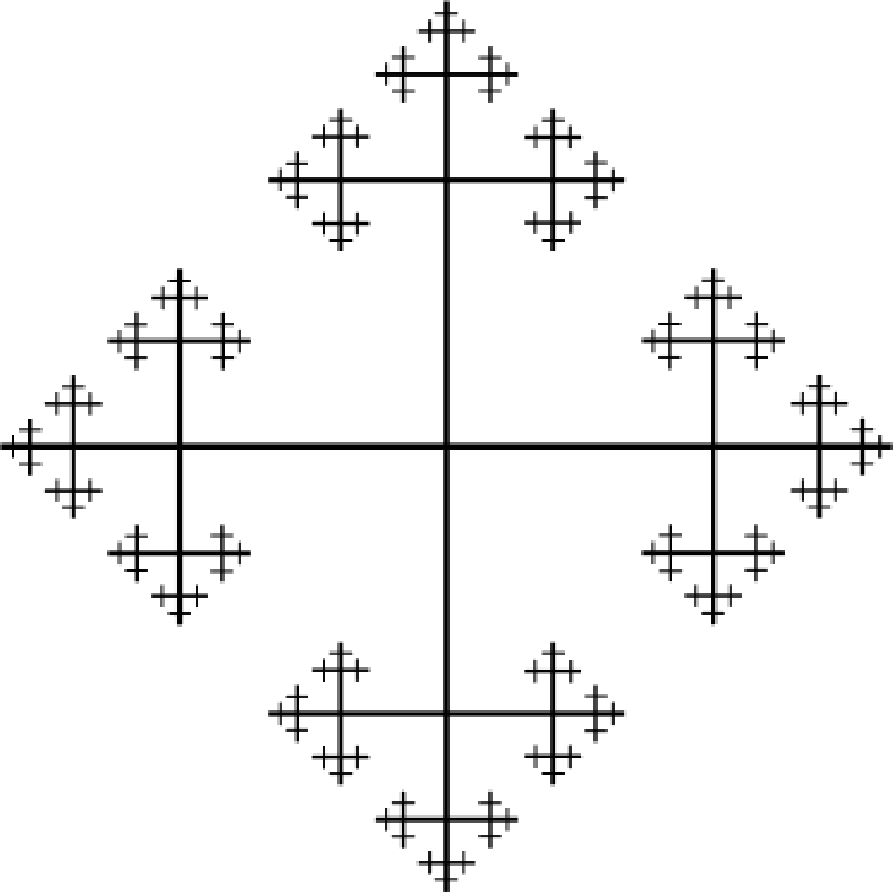
\includegraphics[width=0.25\linewidth]{images/fig8.png}}

	where vertical edges are oriented upwards and labelled by $b$ and horizontal edges are oriented to the right and labelled by $a$. Deck transformations are freely generated by either $D_{a}$ or $D_{b}$, where $D_{a}$ (resp. $D_{b}$) acts on the graph by shifting all edges once to the right, rescaling them appropriately. In other words..
\end{xmp}

\vspace{-7pt}
\begin{thm}[Fundamental Group of \texorpdfstring{$\mathbb{S}^{1} \vee \mathbb{S}^{1}$}{S1 V S1}]{thm:fundamental-group-figeight}{14}
	The fundamental group of $\mathbb{S}^{1} \vee \mathbb{S}^{1}$ is the free group generated by two elements, i.e.
	\vspace{-4pt}
	\[\pi_{1}(\mathbb{S}^{1} \vee \mathbb{S}^{1}) \cong \langle a, b \rangle\]
\end{thm}

\vspace{-7pt}
\begin{xmp}[Covering The M\"obius Band]{xmp:covering-mobius}{20.1}
	Recall the M\"obius band $M : \mathbb{R} \times I / \sim$ is defined by the quotient $(x, y) \sim (x + 1, 1 - y)$. We obtain the homotopy equivalence using covering theory. The quotient map
	\[q : \mathbb{R} \times I \to M\]
	is the universal covering, since $\mathbb{R} \times I$ is simply-connected. For some $n\in \mathbb{Z}$, let $D_{n}$ be the deck transformation:
	\[D_{n} : \mathbb{R} \times I \to \mathbb{R} \times I,\;\quad (x, y) \mapsto (x+n, y_{n})\]
	\par\vspace{-3pt}
	where $y_{n} = y$ if $n$ is even and $y_{n} = 1-y$ for $n$ odd. These are all deck transformations and $\Deck(p)$ is generated by $D_{1}$ since
	\[D_{n} = (D_{1})^{n}\]
	\par\vspace{-3pt}
	\tcbline
	For odd $n$, there are $n$-fold self-coverings $M \to M$. For even $n$, there are $n$-fold coverings by the torus $T^{2} \to M$.
\end{xmp}

\vspace{-7pt}
\begin{xmp}[Covering the Klein Bottle]{xmp:covering-klein-bottle}{20.2}
	Consider the Klein bottle
	\vspace{-4pt}
	\[K = \mathbb{R}^{2} / \sim\]
	where $(x, y) \sim (x + 1, 1 - y) \sim (x, y+1)$ for all $(x, y)\in \mathbb{R}^{2}$. The quotient map
	\vspace{-4pt}
	\[q : \mathbb{R}^{2} \to K\]
	\par\vspace{-3pt}
	is the universal covering map. Consider the deck transformation
	\[D_{a} : \mathbb{R}^{2} \to \mathbb{R}^{2},\;\quad (x, y) \mapsto (x, y+1)\]
	\par\vspace{-3pt}
	and
	\vspace{-3pt}
	\[D_{b} : \mathbb{R}^{2} \to \mathbb{R}^{2},\;\quad (x, y) \mapsto (x+1, 1-y)\]
	\par\vspace{-3pt}
	These two deck transformations generate the deck transformation group $\Deck(q)$ and satisfy the relation:
	\vspace{-3pt}
	\[D_{b} \circ D_{a} \circ D_{b}^{-1} \circ D_{a} = \Id.\]
\end{xmp}

\vspace{-7pt}
\begin{ppn}[Fundamental Group of the Klein Bottle]{ppn:fundamental-group-klein}{10}
	The fundamental group of the Klein Bottle is:
	\vspace{-2pt}
	\[\pi_{1}(K) = \langle a, b \rangle / \langle aba^{-1}b \rangle\]
\end{ppn}


\newpage
\section{Unexaminable Material}
\begin{thm}[Seifert-Vam Kampen Theorem]{thm:seifert}{15}
	Let $X$ be a topological space with a fixed point $x_{0}$. Let $\{U_{\alpha}\}_{\alpha}$ be an open cover of $X$ consisting of path-connected open sets $U_{\alpha}$ containing the fixed point $x_{0}$. The inclusions $U_{\alpha} \subset X$ induce a group homomorphism:
	\[\Phi : \ast_{\alpha} \pi_{1}(U_{\alpha}) \to \pi_{1}(X).\]
	\begin{enumerate-zero}
	    \item If $U_{\alpha} \cap U_{\beta}$ is path-connected for any $\alpha, \beta$, then $\Phi$ is surjective.
	    \item If $U_{\alpha} \cap U_{\beta} \cap U_{\gamma}$ is path-connected for any $\alpha, \beta, \gamma$, then the kernel of $\Phi$ is generated by elements $i_{\alpha\beta}(w) i_{\beta\alpha}(w)^{-1}$ where $w \in \pi_{1}(U_{\alpha} \cap U_{\beta})$ and $i_{\alpha\beta} : \pi_{1}(U_{\alpha} \cap U_{\beta}) \to \pi_{1}(U_{\alpha})$ is the induced homomorphism from the inclusion $U_{\alpha} \cap U_{\beta} \subset U_{\alpha}$.
	\end{enumerate-zero}

	The assumption $U_{\alpha} \cap U_{\beta}$ are path-connected ensures that words $\pi_{1}(U_{\alpha})$ generate $\pi_{1}(X)$. The assumption $U_{\alpha} \cap U_{\beta} \cap U_{\gamma}$ is path-connected gives a presentation for the group $\pi_{1}(X)$.
\end{thm}

\begin{xmp}[Sifert-Vam Kampen on \texorpdfstring{$\mathbb{S}^{1} \vee \mathbb{S}^{1}$}{S1 V S1}]{xmp:sifert-fig8}{17}
	Consider the figure eight $\mathbb{S}^{1} \vee \mathbb{S}^{1} = \mathbb{S}^{1} \times \{1\} \cup \{1\} \times \mathbb{S}^{1}$ and let
	\[U_{i} : = \mathbb{S}^{1} \vee \mathbb{S}^{1} \backslash \{x_{i}\}\]
	be the complements of the points $x_{1} = (-1,1)$ and $x_{2} = (1, -1)$. The sets $U_{1}$ and $U_{2}$ are open path-connected and cover $\mathbb{S}^{1} \vee \mathbb{S}^{1}$. In fact, they are both homotopy equivalent to the circle $U_{i} \simeq \mathbb{S}^{1}$. Their intersection $U_{1} \cap U_{2}$ is contractible, and applying SVK we find,
	\[\pi_{1}(\mathbb{S}^{1} \vee \mathbb{S}^{1}) \cong \mathbb{Z} \ast \mathbb{Z}.\]
\end{xmp}

\begin{xmp}[Fundamental Group of Wedged Circles]{xmp:fundamental-group-wedged-circles}{18}
	Let $(X_{\alpha}, x_{\alpha})$ be a fIYL of path-connected pointed spaces and consider theier wedge sum
	\[X := \bigvee_{\alpha} X_{\alpha}.\]
	suppose that each $x_{a}:= X_{\alpha} \vee \bigvee_{\beta \ne \alpha} U_{\beta} \subset X$.
	By contractibility of the $U_{\alpha}$'s we have homotopy equivalences $A_{\alpha} \simeq X_{\alpha}$. Moreover, the intersection $A_{\alpha} \cap A_{\beta}$ is contractibel for any $\alpha\ne \beta$. Applying SVK we obtain
	\[\pi_{1}(X) \cong \ast_{\alpha} \pi_{1}(X_{\alpha}).\]
	In particular, the fundamental group of the $n$-th wedge sum of circles is the free group on $n$-generators:
	\setcounter{equation}{22}
	\begin{equation}
		\pi_{1}\left(\bigwedge^{n} \mathbb{S}^{1}\right) \cong \mathbb{Z} \ast \cdots \ast \mathbb{Z} \cong \langle  \alpha_{1},\dots, \alpha_{n} \rangle.
	\end{equation}
\end{xmp}

\columnbreak
\begin{dfn}[CW Complexes]{dfn:cw-complex}{25}
	A special class of topological spaces which are constructed inducively attaching $n$-dimensional disks or $n$-cells are called \textbf{CW complexes}. They are described as follows:
	\begin{enumerate-zero}
	    \item A set $X^{0}$ of \textbf{vertices} or $0$-cells
	    \item Inductively construct the $n$-skeleton $X^{n}$ from $X^{n-1}$ by attaching $n$-dimenaional disks $\mathbb{D}^{n}_{\alpha}$ by attaching maps $\phi_{\alpha} : \partial D^{n}_{\alpha} = \mathbb{S}_{\alpha}^{n-1}\to X^{n-1}$. In other words,
			\[X^{n} = X^{n-1} \amalg_{\phi\alpha} \coprod_{\alpha} D^{n}_{\alpha}.\]
	\end{enumerate-zero}
	Equivalently, a \textbf{CW Complex} is a space $X$ along with a filtration of subspaces
	\[X^{0} \subset \cdots X^{n} \subset X^{n+1} \subset \cdots \subset X\]
	such that $X^{n} \backslash X^{n-1}$ is homeomorphic to a disjoint union of $n$-dimensional open disks, and $X^{0}$ is discrete.
\end{dfn}

\begin{xmp}[Examples of CW Complexes]{xmp:cw-complex}{19}
	\begin{enumerate-zero}
	    \item The Torus $T^{2} = I^{2} / \sim$ can be made into a CW complex with: $X^{0} = \{[(0,0)]\},\, X^{1} = \{[(a, 0)] \mid a\in I\} \cup \{[(0, b)] \mid B \in I\}$ and $X^{2} = T^{2}$. In particular, it has one $0$-cell, two $1$-cell, and one $2$-cell.
		\item The real projective plane $\mathbb{RP}^{2}$ can be made into a CW complex with $X^{0} = \ast,\, X^{1} = \mathbb{RP}^{1} = \mathbb{S}^{1}$ and $X^{2}$ obtained by attaching a $2$-disk to $\mathbb{S}^{1}$ along the quotient map $\mathbb{S}^{1} \to \mathbb{RP}^{1}$
	\end{enumerate-zero}
\end{xmp}

\newpage

\end{multicols*}
\end{document}
